%!TEX root = slides.tex

% 1. Languages
% 2. Deciders
% 3. Big O


\section{Computational complexity}


\begin{frame}{Bubble sort for fixed size input}
  \begin{alertblock}{How many comparisons does bubble sort make for different inputs of the same size?}
    \begin{itemize}
      \item Suppose we have a list with 5 elements.
      \item Best case scenario: list already sorted.
      \item Worst case scenario: list reverse sorted.
    \end{itemize}
    \[ [1,2,3,4,5] \]
    \[ [5,2,1,4,3] \]
    \[ [5,4,3,2,1] \]
  \end{alertblock}
\end{frame}


\begin{frame}{Bubble sort for different sized inputs}
  \begin{alertblock}{How many comparisons does bubble sort make for inputs of increasing length?}
    \begin{itemize}
      \item Suppose we have a list with $n$ elements.
      \item Compare the worst-case scenario for each value of $n$.
    \end{itemize}
    \[ [3,2,1] \]
    \[ [4,3,2,1] \]
    \[ [5,4,3,2,1] \]
    \[ [6,5,4,3,2,1] \]
  \end{alertblock}
\end{frame}


\begin{frame}{Average vs. worst case}
  \begin{table}
    \begin{tabular}{p{2cm}rr}
      Input & Algorithm A & \hspace{1cm} Algorithm B \\
      \hline
      (1,2,3) &  1ms &  1ms \\
      (1,3,2) &  1ms &  5ms \\
      (2,1,3) &  2ms &  4ms \\
      (2,3,1) &  2ms &  5ms \\
      (3,1,2) &  2ms &  5ms \\
      (3,2,1) & 10ms &  4ms \\
      \hline
      Average &  3ms &  4ms \\
      Worst   & 10ms &  5ms
    \end{tabular}
  \end{table}
  \begin{center}
    Would you choose Algorithm A or Algorithm B?
  \end{center}
\end{frame}


\begin{frame}{Terminology of complexity}
  \begin{alertblock}{How does the number of operations change as $n$ increases?}
    \begin{description}
      \item[Linear] Multiply $n$ by a constant, add a constant. (Special category of polynomial time.)
      \item[Polynomial] Multiply $n$ by itself a fixed number of times, multiply by a constant. (Can add such terms together.)
      \item[Exponential] Raise a constant to the power of $n$. (Rate of change is still exponential.)
      \item[Logarithmic] Opposite of exponential.
    \end{description}
  \end{alertblock}
\end{frame}


\begin{frame}[fragile]{Terminology of complexity (graph)}
\begin{center}
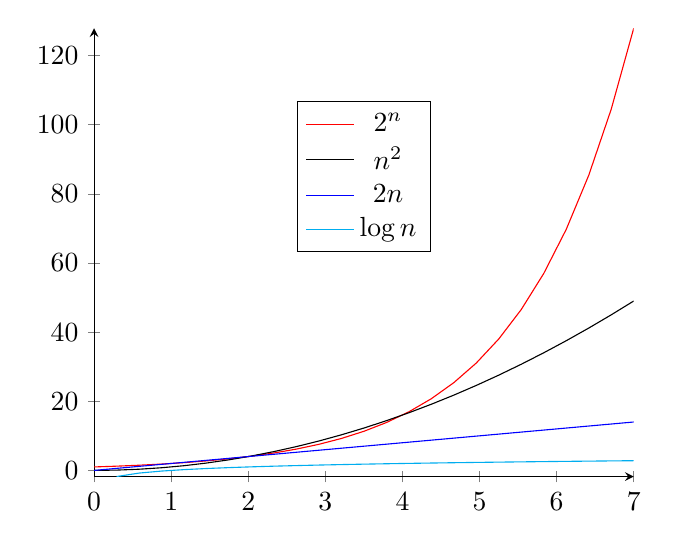
\begin{tikzpicture}
  \begin{axis}[xmin=0, domain=0:7, axis x line=bottom, axis y line=left, legend style={at={(0.5,0.5)},anchor=south}]
    \addplot[red]   {pow(2,x)};
    \addplot[black] {pow(x,2)};
    \addplot[blue]  {2*x};
    \addplot[cyan]  {ln(x)/ln(2))};
    \legend{$2^n$,$n^2$,$2n$,$\log n$};
  \end{axis}
\end{tikzpicture}
\end{center}
\end{frame}


\begin{frame}{Linear}
  \[ f(n) = a_0 + a_1 n \]
  \begin{alertblock}{How many pairs of shoes does a centipede need?}
    \begin{itemize}
      \item Let's say a centipede has 100 feet.
      \item Then every centipede needs 100 shoes.
      \item That's 50 pairs of shoes.
      \item So 2 centipedes need 100 pairs, 3 need 150 pairs, etc.
      \item So $n$ centipedes need $50n$ pairs of shoes.
      \item Linearity is familiar, and most people's default assumption.
      \item You take the input, multiply by a constant, and add another constant.
    \end{itemize}
  \end{alertblock}
\end{frame}


\begin{frame}{Polynomial}
  \[ f(n) = a_0 + a_1 n + a_2 n^2 + a_3 n^3 + \ldots \]
  \begin{alertblock}{What is the volume of a cube of side $n$?}
    \begin{itemize}
      \item Suppose we have a cube with sides of length 1 metre.
      \item The volume of the cube is $1 \times 1 \times 1 = 1$ metres cubed.
      \item Suppose the cube has sides of length 2 metres instead.
      \item The volume of the cube is $2 \times 2 \times 2 = 8$ metres cubed.
      \item In general, for sides of length $n$, the volume is $n^3$.
    \end{itemize}
  \end{alertblock}
\end{frame}


\begin{frame}{Exponential}
  \[ f(n) = a^n \]
  \begin{alertblock}{How many numbers can we represent with $n$ bits?}
    \begin{itemize}
      \item Consider the case of four bits -- imagine four placeholders \textbf{\fbox{?}}\textbf{\fbox{?}}\textbf{\fbox{?}}\textbf{\fbox{?}}
      \item Each placeholder can contain either 0 or 1.
      \item There are $2 \times 2 \times 2 \times 2 = 2^4 = 16$ different numbers.
      \item Add another bit, how many numbers is it now?
      \item It's $2 \times 2 \times 2 \times 2 \times 2 = 2^5 = 32$.
      \item Generally $n$ bits can represent $2^n$ numbers.
    \end{itemize}
  \end{alertblock}
\end{frame}


\begin{frame}{Logarithmic}
  \[ f(n) = \log_a n \]
  \begin{alertblock}{How many bits do we need to represent $n$ numbers?}
    \begin{itemize}
      \item If we have $n$ bits we can represent $2^n$ numbers.
      \item If we want to represent $n$ numbers, how many bits to we need (at a minimum)?
      \item The inverse operation to exponentiation is logarithm.
      \item Remember, $a^n = b$ means $\log_a b = n$.
    \end{itemize}
  \end{alertblock}
\end{frame}

\begin{frame}{Big-O (Sipser)}
  \begin{definition}
    Let $f$ and $g$ be functions $f,g: \mathbb{N} \rightarrow \mathbb{R}^+$.
    We say that $f(n) = O(g(n))$, or $f$ is \emph{big-O} of $g$, if positive integers $c$ and $n_0$ exist such that, for every integer $n$ greater than or equal to $n_0$, $f(n) \le cg(n)$.
  \end{definition}
  \begin{alertblock}{Example}
    Let $f$ be the function $f(n) = 5n^3 + 2n^2 + 22n + 6$.
    We'll prove that $f$ is big-O of $n^3$ ($f = O(n^3)$).
    Let $c$ be $6$ and $n_0$ be $10$.
    Is the following true, for all $n$ greater than or equal to 10, $5n^3 + 2n^2 + 22n + 6 \le 6n^3$?
    Note that as $n$ increases ($n=10,n=11,n=12,\ldots$), $f(n)$ also increases.
    Also note that $f(10) = 5426$ and $6g(10) = 6000$.
  \end{alertblock}
  \citeurl{math.mit.edu/~sipser/book.html}
\end{frame}


\begin{frame}[fragile]{Big-O example graph}
\begin{center}
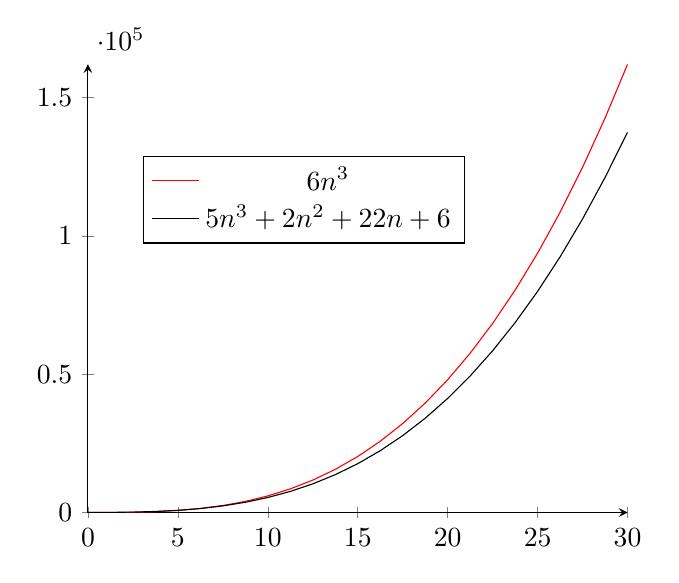
\begin{tikzpicture}
  \begin{axis}[xmin=0, domain=0:30, axis x line=bottom, axis y line=left, legend style={at={(0.4,0.6)},anchor=south}]
    \addplot[red]   {6*pow(x,3)};
    \addplot[black] {5*pow(x,3) + 2*pow(x,2) + 22*x + 6};
    \legend{$6n^3$,$5n^3 + 2n^2 + 22n + 6$};
  \end{axis}
\end{tikzpicture}
\end{center}
\end{frame}

\begin{frame}[fragile]{Smaller values of $n$}
\begin{center}
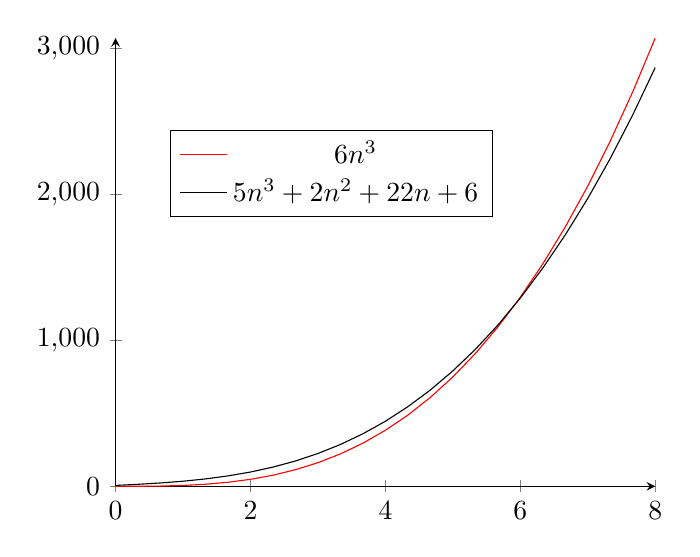
\begin{tikzpicture}
  \begin{axis}[xmin=0, domain=0:8, axis x line=bottom, axis y line=left, legend style={at={(0.4,0.6)},anchor=south}]
    \addplot[red]   {6*pow(x,3)};
    \addplot[black] {5*pow(x,3) + 2*pow(x,2) + 22*x + 6};
    \legend{$6n^3$,$5n^3 + 2n^2 + 22n + 6$};
  \end{axis}
\end{tikzpicture}
\end{center}
\end{frame}

\begin{frame}[fragile]{Bubble sort is $O(n^2)$}
\begin{center}
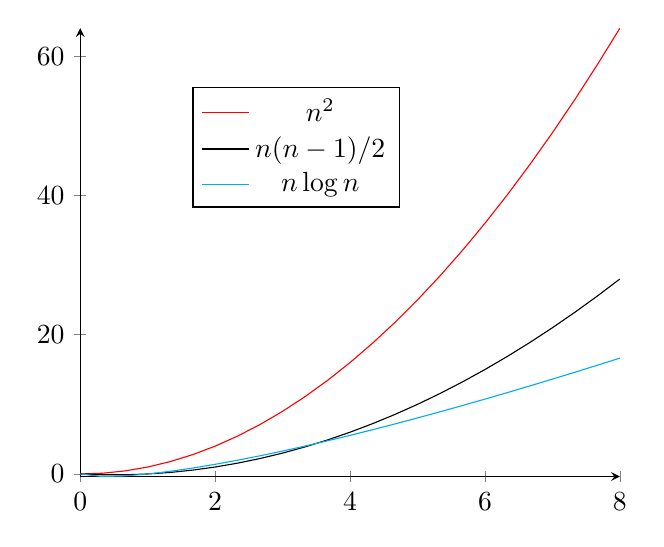
\begin{tikzpicture}
  \begin{axis}[xmin=0, domain=0:8, axis x line=bottom, axis y line=left, legend style={at={(0.4,0.6)},anchor=south}]
    \addplot[red]   {x^2};
    \addplot[black] {x*(x-1)/2};
    \addplot[cyan]   {x*ln(x)};
    \legend{$n^2$,$n(n-1)/2$,$n \log n$};
  \end{axis}
\end{tikzpicture}
\end{center}
\end{frame}


\begin{frame}{Polynomial time}
  \begin{definition}
    An algorithm is said to be solvable in \emph{polynomial time} if the number of steps required to complete the algorithm for a given input is $O(n^k)$ for some nonnegative integer $k$, where $n$ is the complexity of the input.
  \end{definition}
  \vspace{4mm}
  \begin{alertblock}{Informally: P complexity class}
    The P complexity class is the set of problems for which there exists, for each such problem, at least one algorithm to solve that problem in polynomial time.
  \end{alertblock}
\end{frame}


\begin{frame}{Polynomial time on a Turing machine}
  \begin{description}
    \item[Sorting] algorithms are usually compared in terms of comparisons.
    \item[Other algorithms] might be compared in terms of something else, like iterations.
    \item[With Turing machines] we can use the number of times we look up the state table.
    \item[The size] of the input can be the length of the input on the tape initially.
  \end{description}
  \vspace{4mm}
  \begin{alertblock}{P complexity class}
    The P complexity class is the set of languages for which there exists some Turing machine that decides the language in polynomial time.
  \end{alertblock}
\end{frame}


\begin{frame}{Recap on Languages}
  \begin{description}
    \item[Alphabet] Finite set of symbols, denoted $\Sigma$.
    \item[String] Sequence of symbols, $w$ from $\Sigma$.
    \item[Language] Set of strings, denoted $L$.
    \item[Length] Of a string, denoted $|w|$  .
    \item[Empty string] Unique string of length 0, denoted $\epsilon$.
  \end{description}
\end{frame}


\begin{frame}{Kleene star}
  \begin{description}
    \item[Word concatenation:] $w_1 w_2$ is the concatenation of strings $w_1$ and $w_2$.
    \item[String concatenation:] $L_1 L_2$ is the language resulting from the concatenation of all strings in $L_1$ and all words in $L_2$, in that order.
    \item[Powers:] $L^0 = \{ \lambda \}$, $L^1 = L$ and $L^{n+1} = L^n L$ for all $n > 1$.
  \end{description}
  \vspace{0.5cm}
  \begin{block}{Kleene Star}
     \[ L^* =  \bigcup_{i=0}^{\infty} L^i \]
  \end{block}
  Note that treating the alphabet $\Sigma$ as a language in itself, we get that $\Sigma^*$ is the set of all words over $\Sigma$.
\end{frame}


\begin{frame}{Example}
  \begin{description}
    \item[$\Sigma$] $\{ 0, 1 \}$
    \item[$L$] $\{ 00, 01, 10, 11 \}$
    \item[$w_1$] $01$
    \item[$w_3$] $11$
    \item[$w_1 w_3$] $0111$
    \item[$\Sigma^*$] $\{ \lambda, 0, 1, 00, 01, 10, 11, 001, 010, \ldots \}$
    \item[$L^*$] $\{ \lambda, 00, 01, 10, 11, 0000, 0001, \ldots \}$
    \item[$L^+$] $\{ 00, 01, 10, 11, 0000, 0001, \ldots \}$
  \end{description}
\end{frame}

\begin{frame}{Think about $\{0,1\}^*$}
  Consider the set:
  \[ \Sigma^* \quad \textrm{where} \quad \Sigma = \{0,1\} \]
  \vspace{1mm}
  \begin{description}
    \item[$\Sigma^*$]  is the set of all strings (of all lengths) of 0's and 1's.
    \item[Documents] on a computer are elements of $\Sigma^*$.
    \item[Programs] on a computer are elements of $\Sigma^*$.
    \item[The entire contents] of your hard drive is one big string of 0's and 1's, and so is in $\Sigma^*$.
  \end{description}
\end{frame}

\begin{frame}[fragile]{Example of a text file}
Create a text file on your computer with this single line of text:
  \begin{minted}{text}
Hello I'm a text file!
  \end{minted}
  Then open it in a hex editor and see this:
  \begin{minted}{text}
48656C6C6F2049276D206120746578742066696C6521
  \end{minted}
  The hex editor is just displaying the binary as hex:
  \begin{minted}{text}
01001000011001010110110001101100011011110010
00000100100100100111011011010010000001100001
00100000011101000110010101111000011101000010
00000110011001101001011011000110010100100001
  \end{minted}
\end{frame}


\begin{frame}{Decision problems}
  \begin{description}
    \item[Decision problems] are problems where the answer is 0 or 1.
    \[ f:\{0,1\}^n \rightarrow \{0,1\} \]
    \item[Turing machines] model decision problems by deciding languages.
    \vspace{0.1cm}
    \item[Deciders] are Turing machines that decide languages -- they end in an accept or fail state no matter what the input, as opposed to never finishing.
    \vspace{0.1cm}
    \item[Accept] is 1, fail is 0.
  \end{description}
\end{frame}

\begin{frame}{Deciding Word documents}
  \begin{alertblock}{Can a Turing machine decide valid Word documents?}
    Word documents are just strings of 0's and 1's, elements of $\{0,1\}^*$.
    Not all strings of 0's and 1's are valid Word documents.
    
    If you try to open any old string of 0's and 1's in Word, it will likely tell you your file is corrupt.
    
    Can we construct a Turing machine that accepts all valid Word documents, and fails otherwise?
    
    Word seems to be able to decide what a valid Word document is, but it's always dealing with finite inputs.
    The specification might allow for infinite Word documents.
  \end{alertblock}
\end{frame}

\begin{frame}{PRIMES}
  \begin{definition}
    $$ PRIMES = \{ 2, 3, 5, 7, 11, 13, ... \} $$
  \end{definition}
  \begin{description}
    \item[PRIMES] is the set of all primes numbers.
    \item[Can] a Turing Machine be designed to decide PRIMES? (Yes)
    \item[Some] people say PRIMES is the decision problem for the set of primes.
    \item[Can] it do it in polynomial time? (Yes)
    \item[Is] PRIMES in P? (Yes, 2002)
  \end{description}
  \citeurl{www.cse.iitk.ac.in/users/manindra/algebra/primality\_v6.pdf}
\end{frame}

\begin{frame}{Modern cryptography}
  \begin{alertblock}{Modern asymmetric key cryptography is based on prime numbers}
    It depends on two facts:
    \begin{itemize}
      \item It's easy to verify primes (P).
      \item It's hard to decompose a composite number into primes (Not known to be P).
    \end{itemize}
  \end{alertblock}
  \begin{alertblock}{Generating versus verifying}
    Note that it's not necessarily easy to generate prime numbers.
    We know that verifying a number is prime can be done in polynomial time.
    That doesn't mean that we can generate prime numbers in polynomial time.
    You must start with the prime, and then ask the question.
  \end{alertblock}

\end{frame}

\begin{frame}[fragile]{Brute force prime checking}
  \begin{alertblock}{Is n a prime?}
    \begin{minted}{c}
function is_prime(n) {
  for (var i = 2; i < n; i++) {
    if (n % i == 0)
      return false;
  }
  return true;
}
    \end{minted}
  \end{alertblock}
\end{frame}

\begin{frame}[fragile]{More efficient prime checking}
  \begin{itemize}
    \item Suppose $a \times b = n$.
    \item Then $a < b$, $a > b$ or $a = b$.
    \item No matter what, $a \le \sqrt{n}$ and/or $b \le \sqrt{n}$.
    \item So only loop to $\sqrt{n}$.
    \item This still isn't that efficient.
  \end{itemize}
\end{frame}

\begin{frame}[fragile]{Slightly more efficient}
  \begin{alertblock}{Is n a prime?}
    \begin{minted}{c}
function is_prime(n) {
  for (var i = 2; i < Math.sqrt(n); i++) {
    if (n % i == 0)
      return false;
  }
  return true;
}
    \end{minted}
  \end{alertblock}
\end{frame}

%\begin{frame}[fragile]{AKS prime checking (2002)}
%  \begin{enumerate}
%    \item If $n = a^b$ where $a,b \in \mathbb{N}^+$, output composite.
%    \item Find the smallest $r$ such that $ord_r(n) > (log_2 n)^2$.
%    \item No matter what, $a \le \sqrt{n}$ and/or $b \le \sqrt{n}$.
%    \item So only loop to $\sqrt{n}$.
%    \item This still isn't that efficient.
%  \end{enumerate}
%  \citeurl{wikipedia.org/wiki/AKS\_primality\_test}
%\end{frame}